%%%%%%%%%%%%%%%%%%%%%%%%%%%%%%%%%%%%%%%%%
% Beamer Presentation
% LaTeX Template
% Version 1.0 (10/11/12)
%
% This template has been downloaded from:
% http://www.LaTeXTemplates.com
%
% License:
% CC BY-NC-SA 3.0 (http://creativecommons.org/licenses/by-nc-sa/3.0/)
%
%%%%%%%%%%%%%%%%%%%%%%%%%%%%%%%%%%%%%%%%%

%----------------------------------------------------------------------------------------
%	PACKAGES AND THEMES
%----------------------------------------------------------------------------------------

\documentclass{beamer}

\mode<presentation> {

% The Beamer class comes with a number of default slide themes
% which change the colors and layouts of slides. Below this is a list
% of all the themes, uncomment each in turn to see what they look like.

%\usetheme{default}
%\usetheme{AnnArbor}
%\usetheme{Antibes}
%\usetheme{Bergen}
%\usetheme{Berkeley}
%\usetheme{Berlin}
%\usetheme{Boadilla}
%\usetheme{CambridgeUS}
%\usetheme{Copenhagen}
%\usetheme{Darmstadt}
%\usetheme{Dresden}
%\usetheme{Frankfurt}
%\usetheme{Goettingen}
%\usetheme{Hannover}
%\usetheme{Ilmenau}
%\usetheme{JuanLesPins}
%\usetheme{Luebeck}
%\usetheme{Madrid}
%\usetheme{Malmoe}
%\usetheme{Marburg}
%\usetheme{Montpellier}
%\usetheme{PaloAlto}
%\usetheme{Pittsburgh}
%\usetheme{Rochester}
\usetheme{Singapore}
%\usetheme{Szeged}
%\usetheme{Warsaw}

% As well as themes, the Beamer class has a number of color themes
% for any slide theme. Uncomment each of these in turn to see how it
% changes the colors of your current slide theme.

%\usecolortheme{albatross}
%\usecolortheme{beaver}
%\usecolortheme{beetle}
%\usecolortheme{crane}
%\usecolortheme{dolphin}
%\usecolortheme{dove}
%\usecolortheme{fly}
%\usecolortheme{lily}
%\usecolortheme{orchid}
\usecolortheme{rose}
%\usecolortheme{seagull}
%\usecolortheme{seahorse}
%\usecolortheme{whale}
%\usecolortheme{wolverine}

%\setbeamertemplate{footline} % To remove the footer line in all slides uncomment this line
%\setbeamertemplate{footline}[page number] % To replace the footer line in all slides with a simple slide count uncomment this line

%\setbeamertemplate{navigation symbols}{} % To remove the navigation symbols from the bottom of all slides uncomment this line
}

\usepackage{graphicx} % Allows including images
\usepackage{booktabs} % Allows the use of \toprule, \midrule and \bottomrule in tables
\usepackage{amsmath}
\usepackage{textcomp}
\usepackage{listings}
\usepackage{xcolor}

\definecolor{commentsColor}{rgb}{0.497495, 0.497587, 0.497464}
\definecolor{keywordsColor}{rgb}{0.000000, 0.000000, 0.635294}
\definecolor{stringColor}{rgb}{0.558215, 0.000000, 0.135316}

\lstset{ %
	backgroundcolor=\color{white},   % choose the background color; you must add \usepackage{color} or \usepackage{xcolor}
	basicstyle=\footnotesize,        % the size of the fonts that are used for the code
	breakatwhitespace=false,         % sets if automatic breaks should only happen at whitespace
	breaklines=true,                 % sets automatic line breaking
	captionpos=b,                    % sets the caption-position to bottom
	commentstyle=\color{commentsColor}\textit,    % comment style
	deletekeywords={...},            % if you want to delete keywords from the given language
	escapeinside={\%*}{*)},          % if you want to add LaTeX within your code
	extendedchars=true,              % lets you use non-ASCII characters; for 8-bits encodings only, does not work with UTF-8
	frame=tb,	                   	   % adds a frame around the code
	keepspaces=true,                 % keeps spaces in text, useful for keeping indentation of code (possibly needs columns=flexible)
	keywordstyle=\color{keywordsColor}\bfseries,       % keyword style
	language=Python,                 % the language of the code (can be overrided per snippet)
	otherkeywords={*,...},           % if you want to add more keywords to the set
	numbers=left,                    % where to put the line-numbers; possible values are (none, left, right)
	numbersep=5pt,                   % how far the line-numbers are from the code
	numberstyle=\tiny\color{commentsColor}, % the style that is used for the line-numbers
	rulecolor=\color{black},         % if not set, the frame-color may be changed on line-breaks within not-black text (e.g. comments (green here))
	showspaces=false,                % show spaces everywhere adding particular underscores; it overrides 'showstringspaces'
	showstringspaces=false,          % underline spaces within strings only
	showtabs=false,                  % show tabs within strings adding particular underscores
	stepnumber=1,                    % the step between two line-numbers. If it's 1, each line will be numbered
	stringstyle=\color{stringColor}, % string literal style
	tabsize=2,	                   % sets default tabsize to 2 spaces
	columns=fixed                    % Using fixed column width (for e.g. nice alignment)
}

\AtBeginSection[]{
	\frame{
		\tableofcontents[currentsection]
	}
}

\AtBeginSubsection[]{
	\frame{
		\tableofcontents[currentsection,currentsubsection]
	}
}




%----------------------------------------------------------------------------------------
%	TITLE PAGE
%----------------------------------------------------------------------------------------

\title{Progetto di Metodi del Calcolo Scientifico} % The short title appears at the bottom of every slide, the full title is only on the title page

\author{Tonelli Lidia Lucrezia (m. 813114)\\
Grassi Marco (m. 830694)\\
Giudice Gianluca (m. 829664)
} % Your name
\institute[University of Milano Bicocca] % Your institution as it will appear on the bottom of every slide, may be shorthand to save space
{
University of Milano Bicocca \\ % Your institution for the title page
\medskip
}
\date{Giugno 2021} % Date, can be changed to a custom date

\begin{document}

\begin{frame}
\titlepage % Print the title page as the first slide
\end{frame}

%----------------------------------------------------------------------------------------
%	PRESENTATION SLIDES
%----------------------------------------------------------------------------------------

%------------------------------------------------
\section{Metodi diretti per matrici sparse}
%------------------------------------------------

\subsection{Approccio al problema}

\begin{frame}
	
	\frametitle{Sistema operativo e hardware }
	Sistema operativo (installazione da zero)
	\begin{itemize}
		\item Windows 10 Pro
		\item Ubuntu 20.04 LTS
	\end{itemize}

	Hardware
	\begin{itemize}
		\item CPU: Intel Core i7-8550U 4 x 1.8 - 4 GHz
		\item RAM: 32 GB, DDR4-2400
	\end{itemize}
\end{frame}


\begin{frame}
	
	\frametitle{Ambienti di programmazione e librerie utilizzate}
	Abbiamo utilizzato 3 ambienti di programmazione; per Python abbiamo usato 3 librerie, di cui una necessaria per ottimizzare il calcolo su matrici molto grandi.
	\begin{itemize}
		\item Matlab  R2021a
		\item GNU Octave 6.1.0
		\item Python 3.8.7
		\begin{itemize}
			\item numpy 1.20.3
			\item scipy 1.6.3
			\item scikit-sparse 0.4.4
		\end{itemize}
	\end{itemize}
	N.B.: Per entrambi i sistemi operativi \'e stata utilizzata la stessa versione di libreria in modo da avere risultati conmparabili.
\end{frame}


\begin{frame}
	\frametitle{Metriche di performance}
	Per misurare le performance sono state utilizzate le seguenti metriche:
	\begin{itemize}
		\item Tempo di calcolo della soluzione
		\item Picco memoria RAM utilizzata per risolvere il sistema
		\item Errore della soluzione: \[err \_ rel = \frac{\|x - xe\|_2}{\|xe\|_2}\]
		con $\| \cdot \|$ la norma euclidea dei vettori
	\end{itemize}
	\end{frame}

\begin{frame}
	
	\frametitle{Tecniche di misurazione}
		\begin{enumerate}
		\item Creazione dei 4 script per il calcolo della soluzione di una matrice
		\begin{itemize}
			\item INPUT: file matrice
			\item OUTPUT: File di report
		\end{itemize}

		\item 10 iterazioni per il calcolo delle misure (in modo tale da avere risultati statisticamente validi)
	
		\begin{itemize}
			\item Scirpt python con funzione di wrapper per profilare la memoria utilizzata.
			\begin{enumerate}
				\item Run di ogni script per ogni matrice su ogni sistema operativo.

					\item Misurazione del tempo (si considera solo il tempo per il calcolo della soluzione)
					\item Misurazione dell'errore 

			\end{enumerate}
			
		\end{itemize}


		\item Analisi dei report generati				

	\end{enumerate}
\end{frame}


\begin{frame}
	
	\frametitle{Tecniche di misurazione}
	
	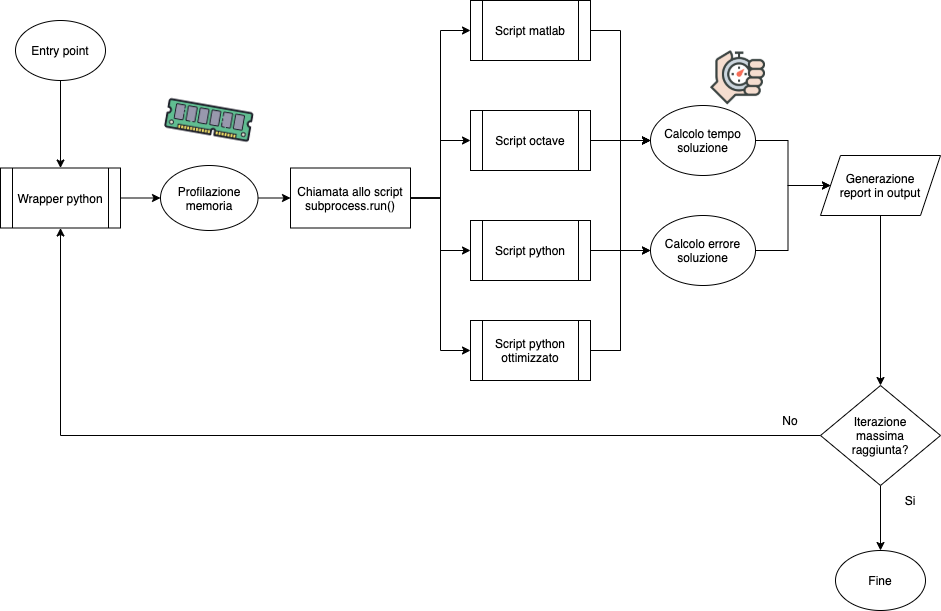
\includegraphics[height=0.6\textwidth]{assets/execution_workflow.png}
	
\end{frame}

\subsection{Analisi delle librerie}

\begin{frame}
	
\frametitle{Matlab}
Matlab \'e ben documentato alla pagina \url{it.mathworks.com/help/matlab}, con motore di ricerca ed esempi.\\
\textbf{Memorizzazione di matrici sparse}: data una matrice sparsa, Matlab salva solo gli elementi diversi da 0 in una lista, insieme al numero di colonna e riga. \\
\textbf{Risoluzione di $Ax = b$}: Matlab ha a disposizione tanti risolutori di sistemi, il cui uso dipende dalla forma della matrice $A$; pertanto, quando viene eseguito il comando $A \setminus b$ si fanno una serie di controlli su $A$, i casi presi in considerazione sono: matrice quadrata, triangolare, triangolare permutata, Hermitiana, Hessenberg superiore, la matrice ha la diagonale tutta positiva o tutta negativa, la matrice \'e simmetrica e definita positiva. In tutti questi casi viene usato un solutore diverso, ad esempio se la matrice \'e simmetrica e definita positiva si applica l'algoritmo di Cholesky.
\end{frame}

\begin{frame}
\frametitle{Octave}
Octave \'e documentato in modo scomodo rispetto a Matlab alla pagina \url{https://octave.org/doc/v6.2.0}, che \'e un semplice manuale. \\
\textbf{Memorizzazione di matrici sparse}: usa il \textit{compressed column format}, ovvero salva solo gli elementi diversi da 0 con il proprio numero di riga, e per ogni colonna salva il numero di elementi diversi da 0 per quella colonna; pertanto al posto di una tripletta per ogni elemento diverso da 0, si salva una coppia e in pi\'u un numero per ogni colonna, ottimizzando la memorizzazione. \\
\textbf{Risoluzione di $Ax = b$}: si comporta allo stesso modo di Matlab, ovvero considera la forma della matrice $A$ per scegliere il risolutore adatto. Anche Octave, come Matlab, prova ad applicare Cholesky e se non riesce significa che la matrice non \'e definita positiva e/o simmetrica.
\end{frame}

\begin{frame}
\frametitle{Python (\textit{numpy} + \textit{scipy} + \textit{scikit-sparse})}
Python è un linguaggio di programmazione general purpose. Abbiamo utilizzato 3 librerie apposite per il calcolo scientifico, ognuna con un compito diverso.
\begin{enumerate}
\item \textit{numpy}: libreria utilizzata per leggere e gestire le matrice in memoria
\item \textit{scipy}: libreria specifica per il calcolo scientifico. Utilizza metodi diretti per il calcolo della soluzione di un sistema.\\
Il metodo standard per la risoluzione diretta di sistemi lineari non \'e ottimizzato come in Matlab o Octave, ovvero non divide i risolutori in base alla matrice. Supporta la fattorizzazione LU tuttavia non \'e abilitata di default; non supporta Cholesky su matrici sparse.
\item \textit{scikit-sparse}: libreria che permette di applicare Cholsesky su matrici sparse; \'e implementata in c.
\end{enumerate}
\end{frame}
\begin{frame}
\frametitle{Python (\textit{numpy} + \textit{scipy} + \textit{scikit-sparse})}
\textit{numpy} e \textit{scipy} \'e documentato peggio di Matlab ma meglio di Octave: ci sono molti esempi ed \'e disponibile il codice essendo open source, anche non essendo presente una buona spiegazione del workflow come in Matlab, si pu\'o capire leggendo il codice; la documentazione si trova alla pagina \url{https://www.scipy.org/docs.html}.\\ \textit{sciki-sparse} non ha una documentazione chiara, ma anche in questo caso, essendo open source, \'e possibile leggere direttamente il codice; la documentazione si trova alla pagina \url{https://scikit-sparse.readthedocs.io/en/latest/cholmod.html}.
\end{frame}
\begin{frame}
\frametitle{Python (\textit{numpy} + \textit{scipy} + \textit{scikit-sparse})}
\textbf{Memorizzazione di matrici sparse}: \textit{numpy} salva le matrici sparse come Matlab.\\
\textbf{Risoluzione di $Ax = b$}: il risolutore assume che la soluzione $x$ sia sparsa, perch\'e pu\'o capitare spesso; se invece $x$ \'e densa, la costruzione risulta molto pi\'u costosa. Utilizza sempre la fattorizzazione LU per risolvere il sistema, quindi il suo comportamento non \'e differente nel caso di matrici simmetriche e definite positive, perch\'e non utilizza mai Cholesky; per questo motivo abbiamo introdotto la libreria \textit{scikit-sparse}, che permette di applicare Cholesky a grandi matrici sparse, perci\'o abbiamo potuto adattare l'algoritmo scritto in Python ai casi di matrici simmetriche e definite positive.
\end{frame}

\begin{frame}
\frametitle{Nuovo workflow con \textit{scikit-sparse}}
\end{frame}

%------------------------------------------------
\subsection{Campagna sperimentale}

\begin{frame}
\frametitle{Propriet\'a delle matrici}
\begin{table}
\begin{tabular}{c c c c}
\toprule
\textbf{Matrice} & \textbf{Simmetrica} & \textbf{Def. pos.} & \textbf{Cand. Cholesky}\\
\midrule
Hook$\_$1498 & Y & Y & Y\\
 G3$\_$circuit & Y & Y & Y\\
 nd24k & Y & Y & Y\\
 boundle$\_$adj & Y & Y & Y\\
 ifiss$\_$mat & N & N & N\\
 TSC$\_$OPF$\_$1047 & Y & N & N\\
 ns3Da & N & N & N\\
 GT01R & N & N & N \\
\bottomrule
\end{tabular}
\end{table}
Durante l'esecuzione di ogni script si suppone di non essere a conoscenza di queste informazioni, cos\'i da rimanere il pi\'u generali possibili.
\end{frame}

\begin{frame}
	\frametitle{Dimensione delle matrici}
	\begin{figure}
		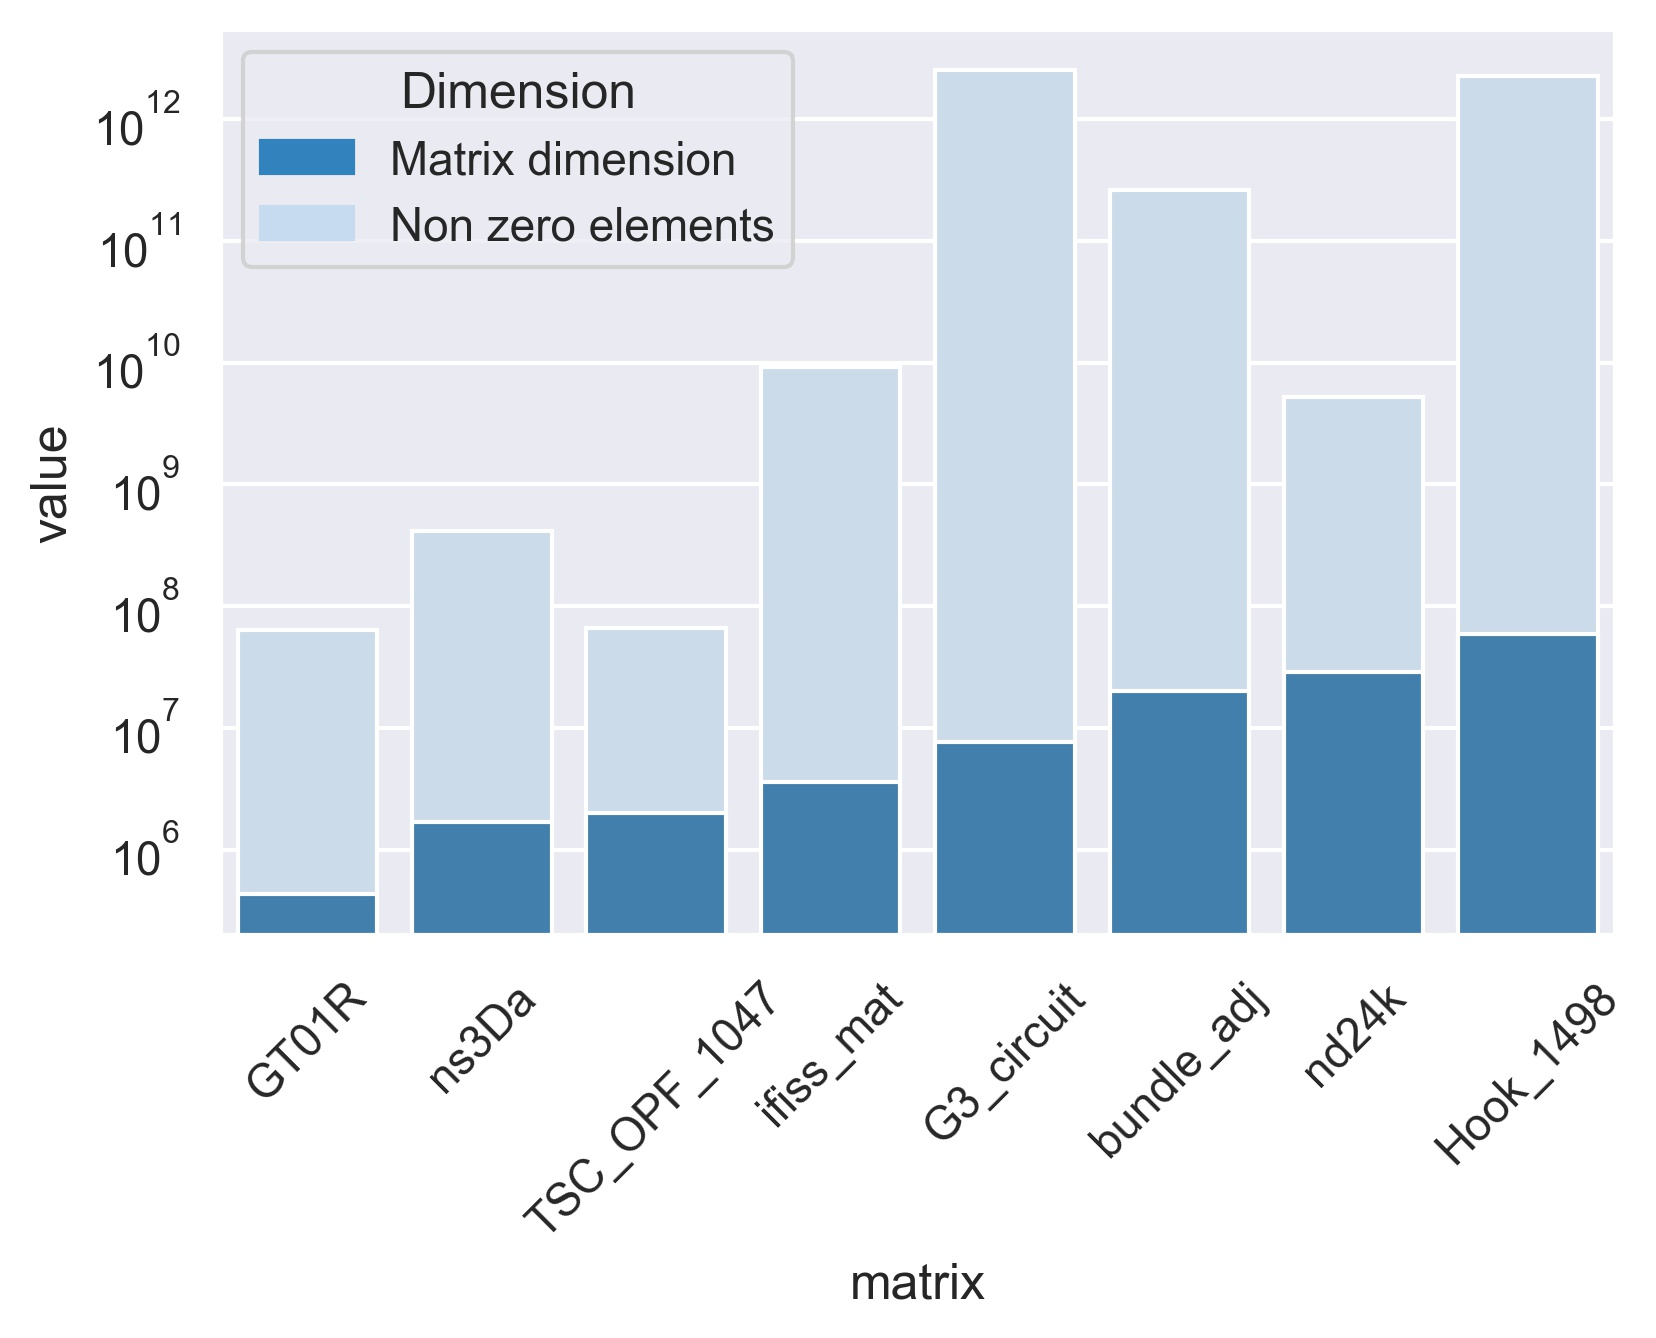
\includegraphics[width=0.8\textheight]{assets/dimension2.jpg}
		\caption{Confronto delle dimensioni e del numero di nnz delle matrici.}
		\label{fig:dim}
	\end{figure}
\end{frame}

\begin{frame}
\frametitle{Grafici performance}
Confronto tra Matlab,  Octave, Python su Windows o Linux per i parametri velocità, precisione e occupazione di memoria.
\end{frame}


\begin{frame}
	\frametitle{Tempo di esecuzione}
	\begin{figure}
		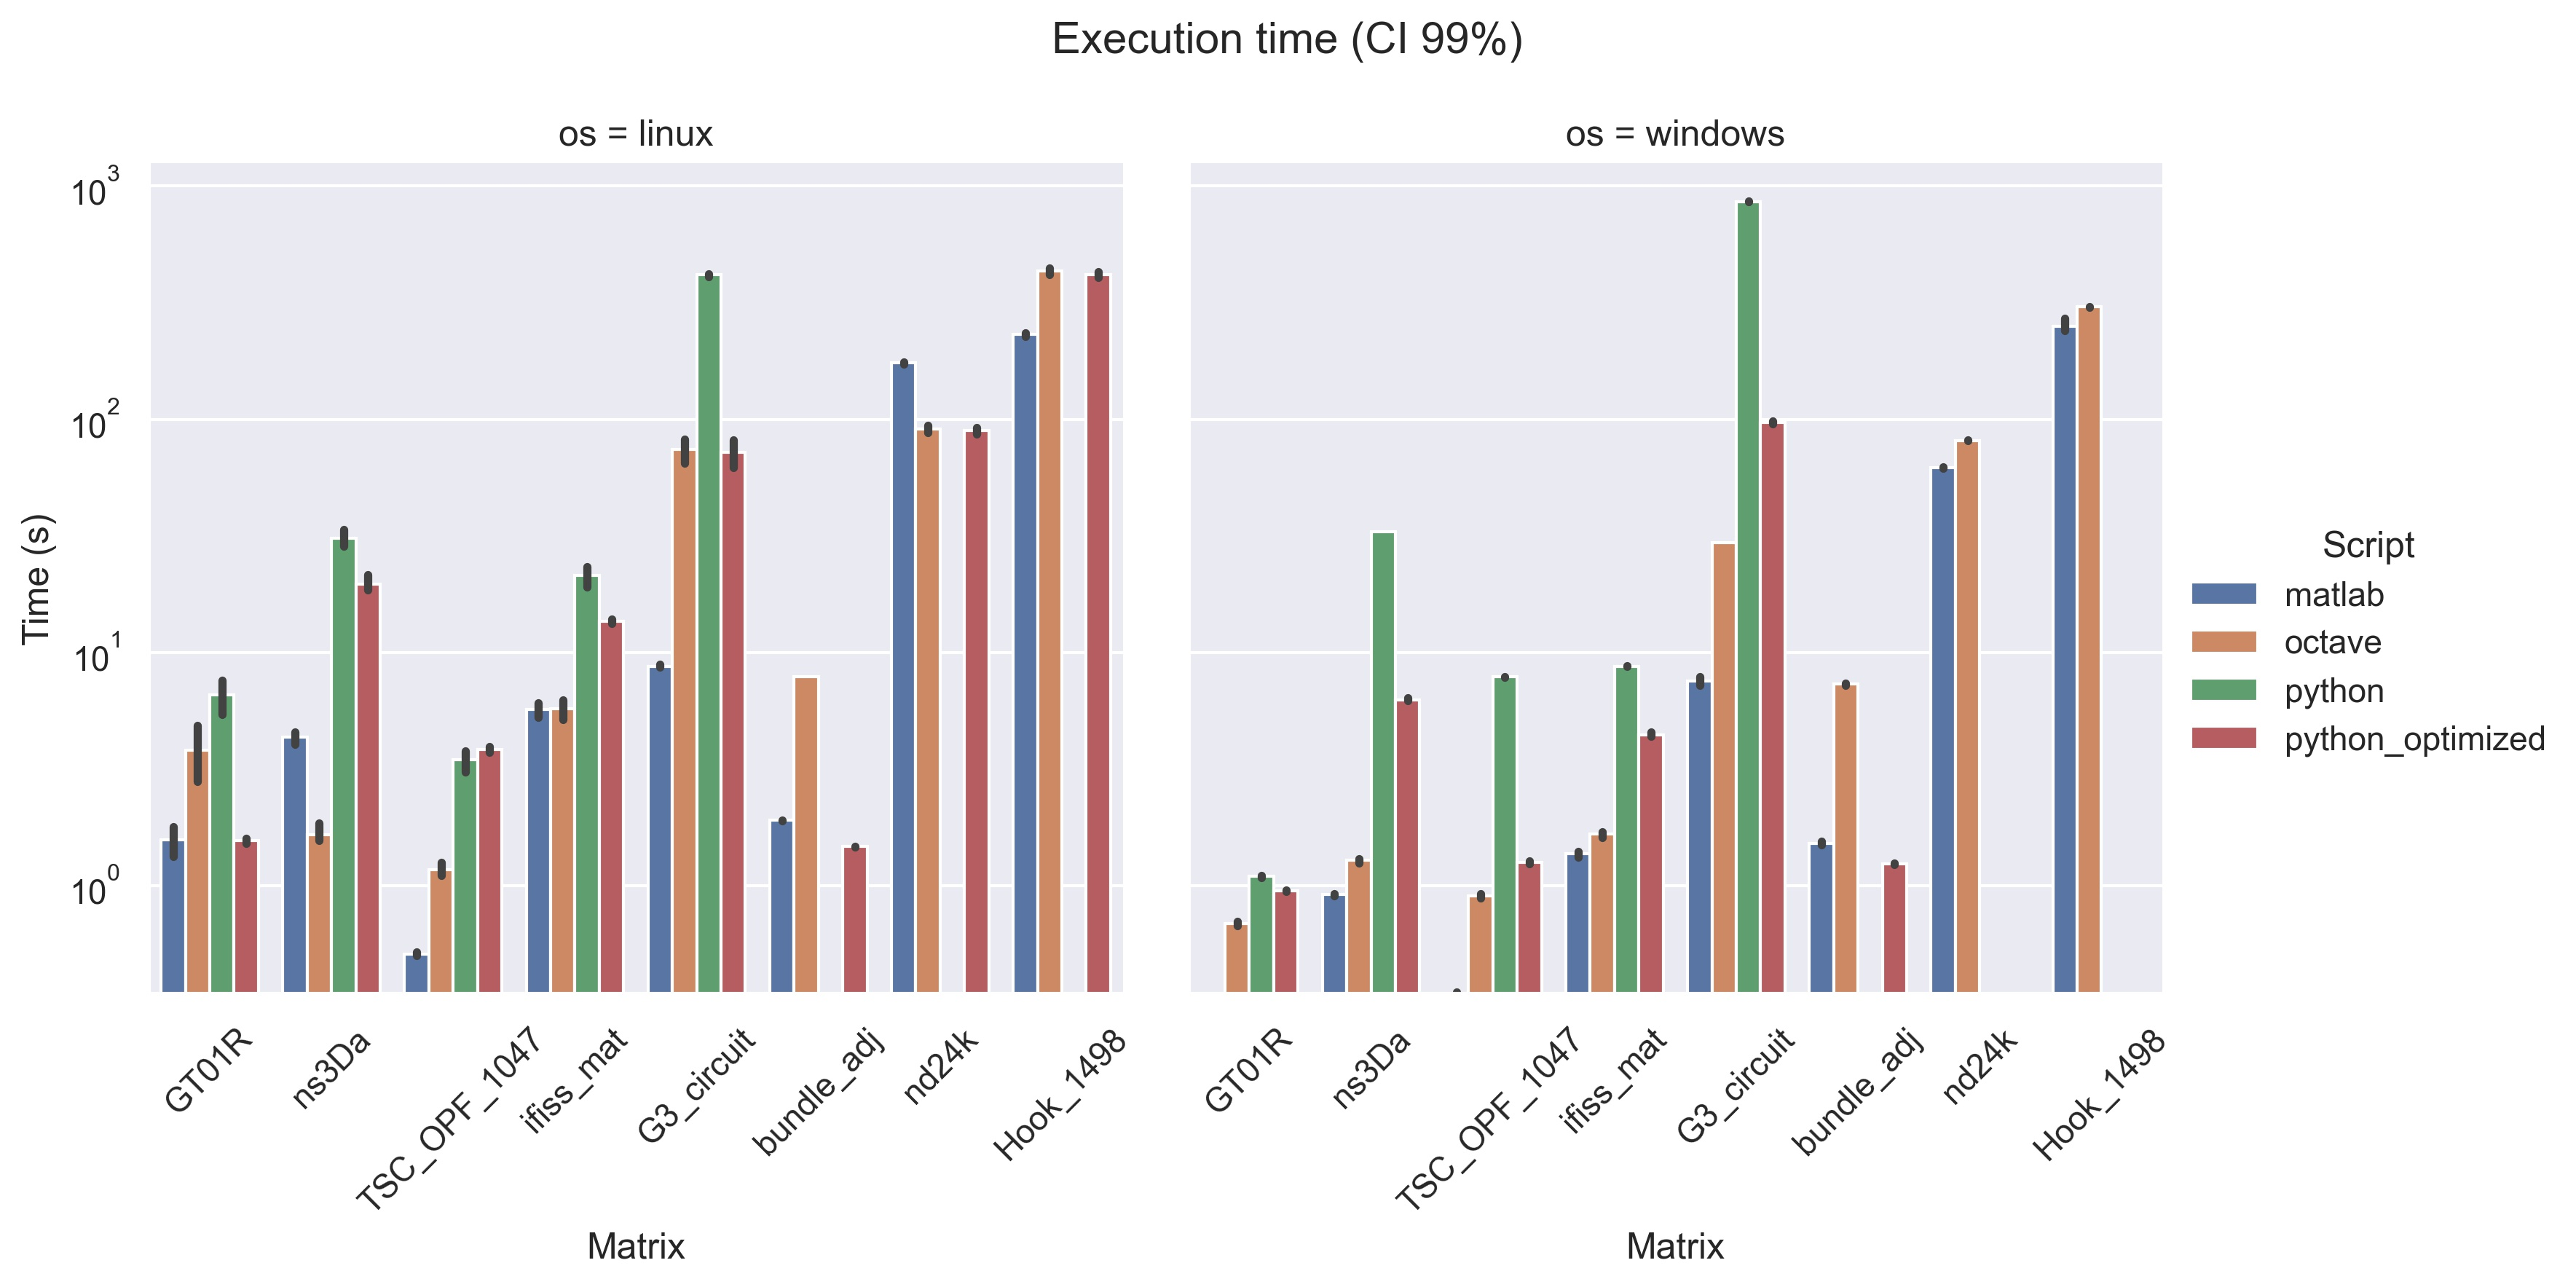
\includegraphics[width=1.35\textheight]{assets/execution.jpg}
		\caption{Confronto tempo di esecuzione.}
		\label{fig:execution}
	\end{figure}
\end{frame}

\begin{frame}
	\frametitle{Memoria utilizzata}
	\begin{figure}
		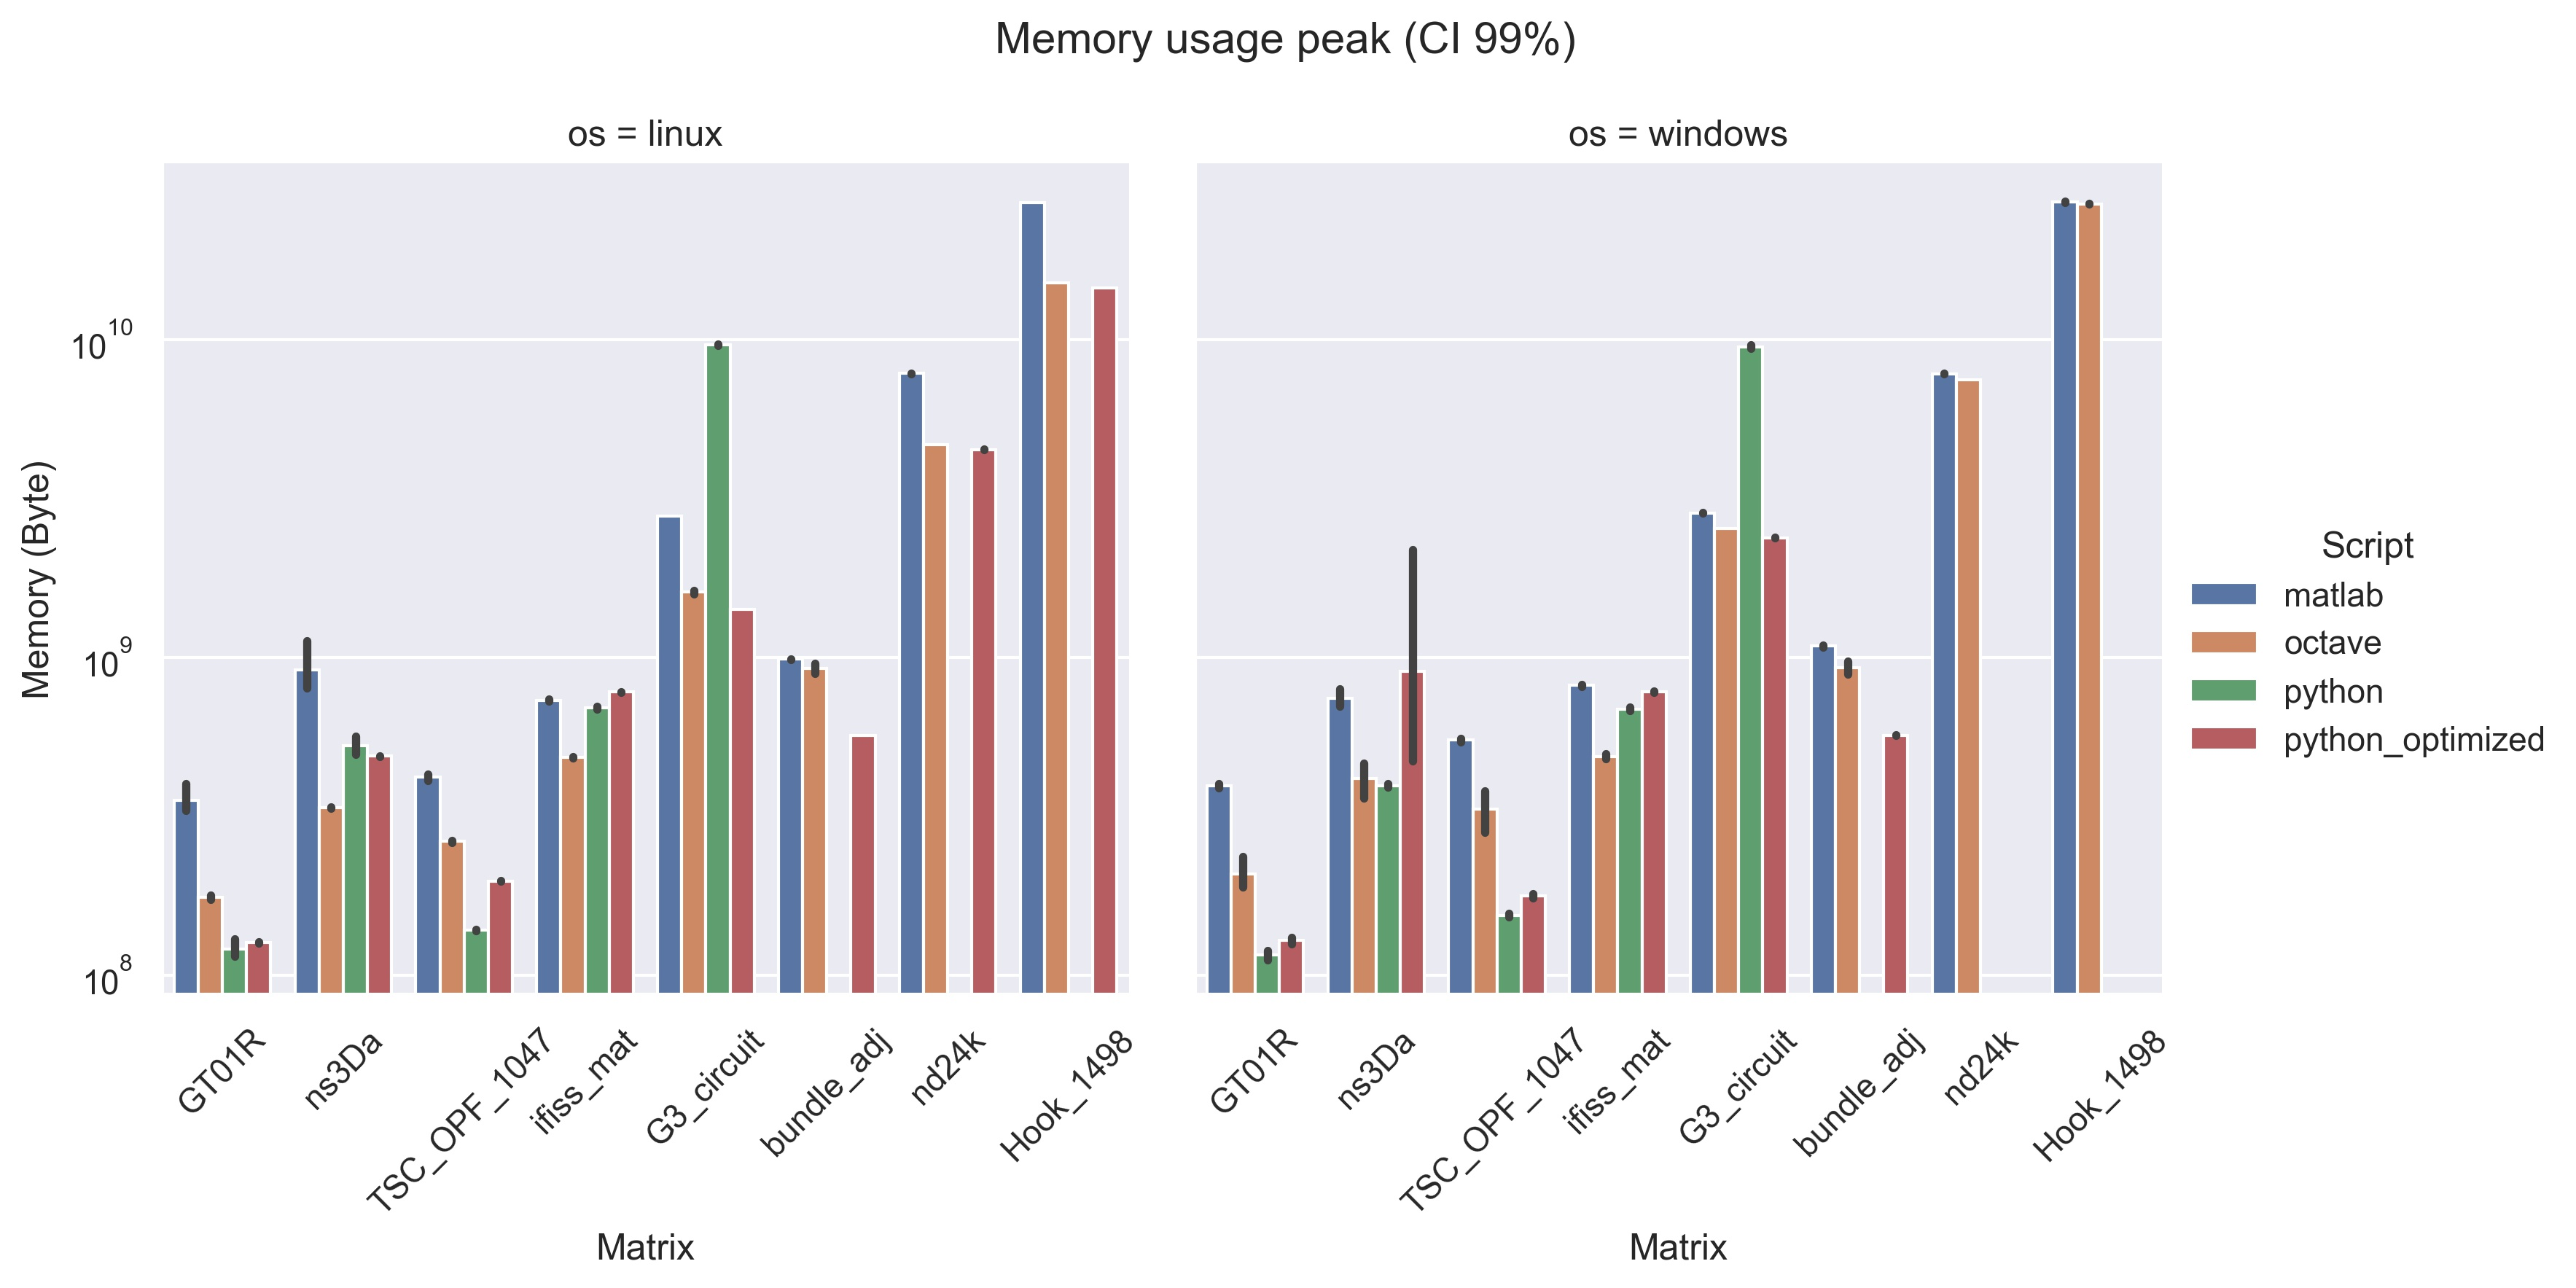
\includegraphics[width=1.35\textheight]{assets/memory.jpg}
		\caption{Picco di memoria utilizzata (in byte).}
		\label{fig:memory}
	\end{figure}
\end{frame}

\begin{frame}
	\frametitle{Tempo di esecuzione}
	\begin{figure}
		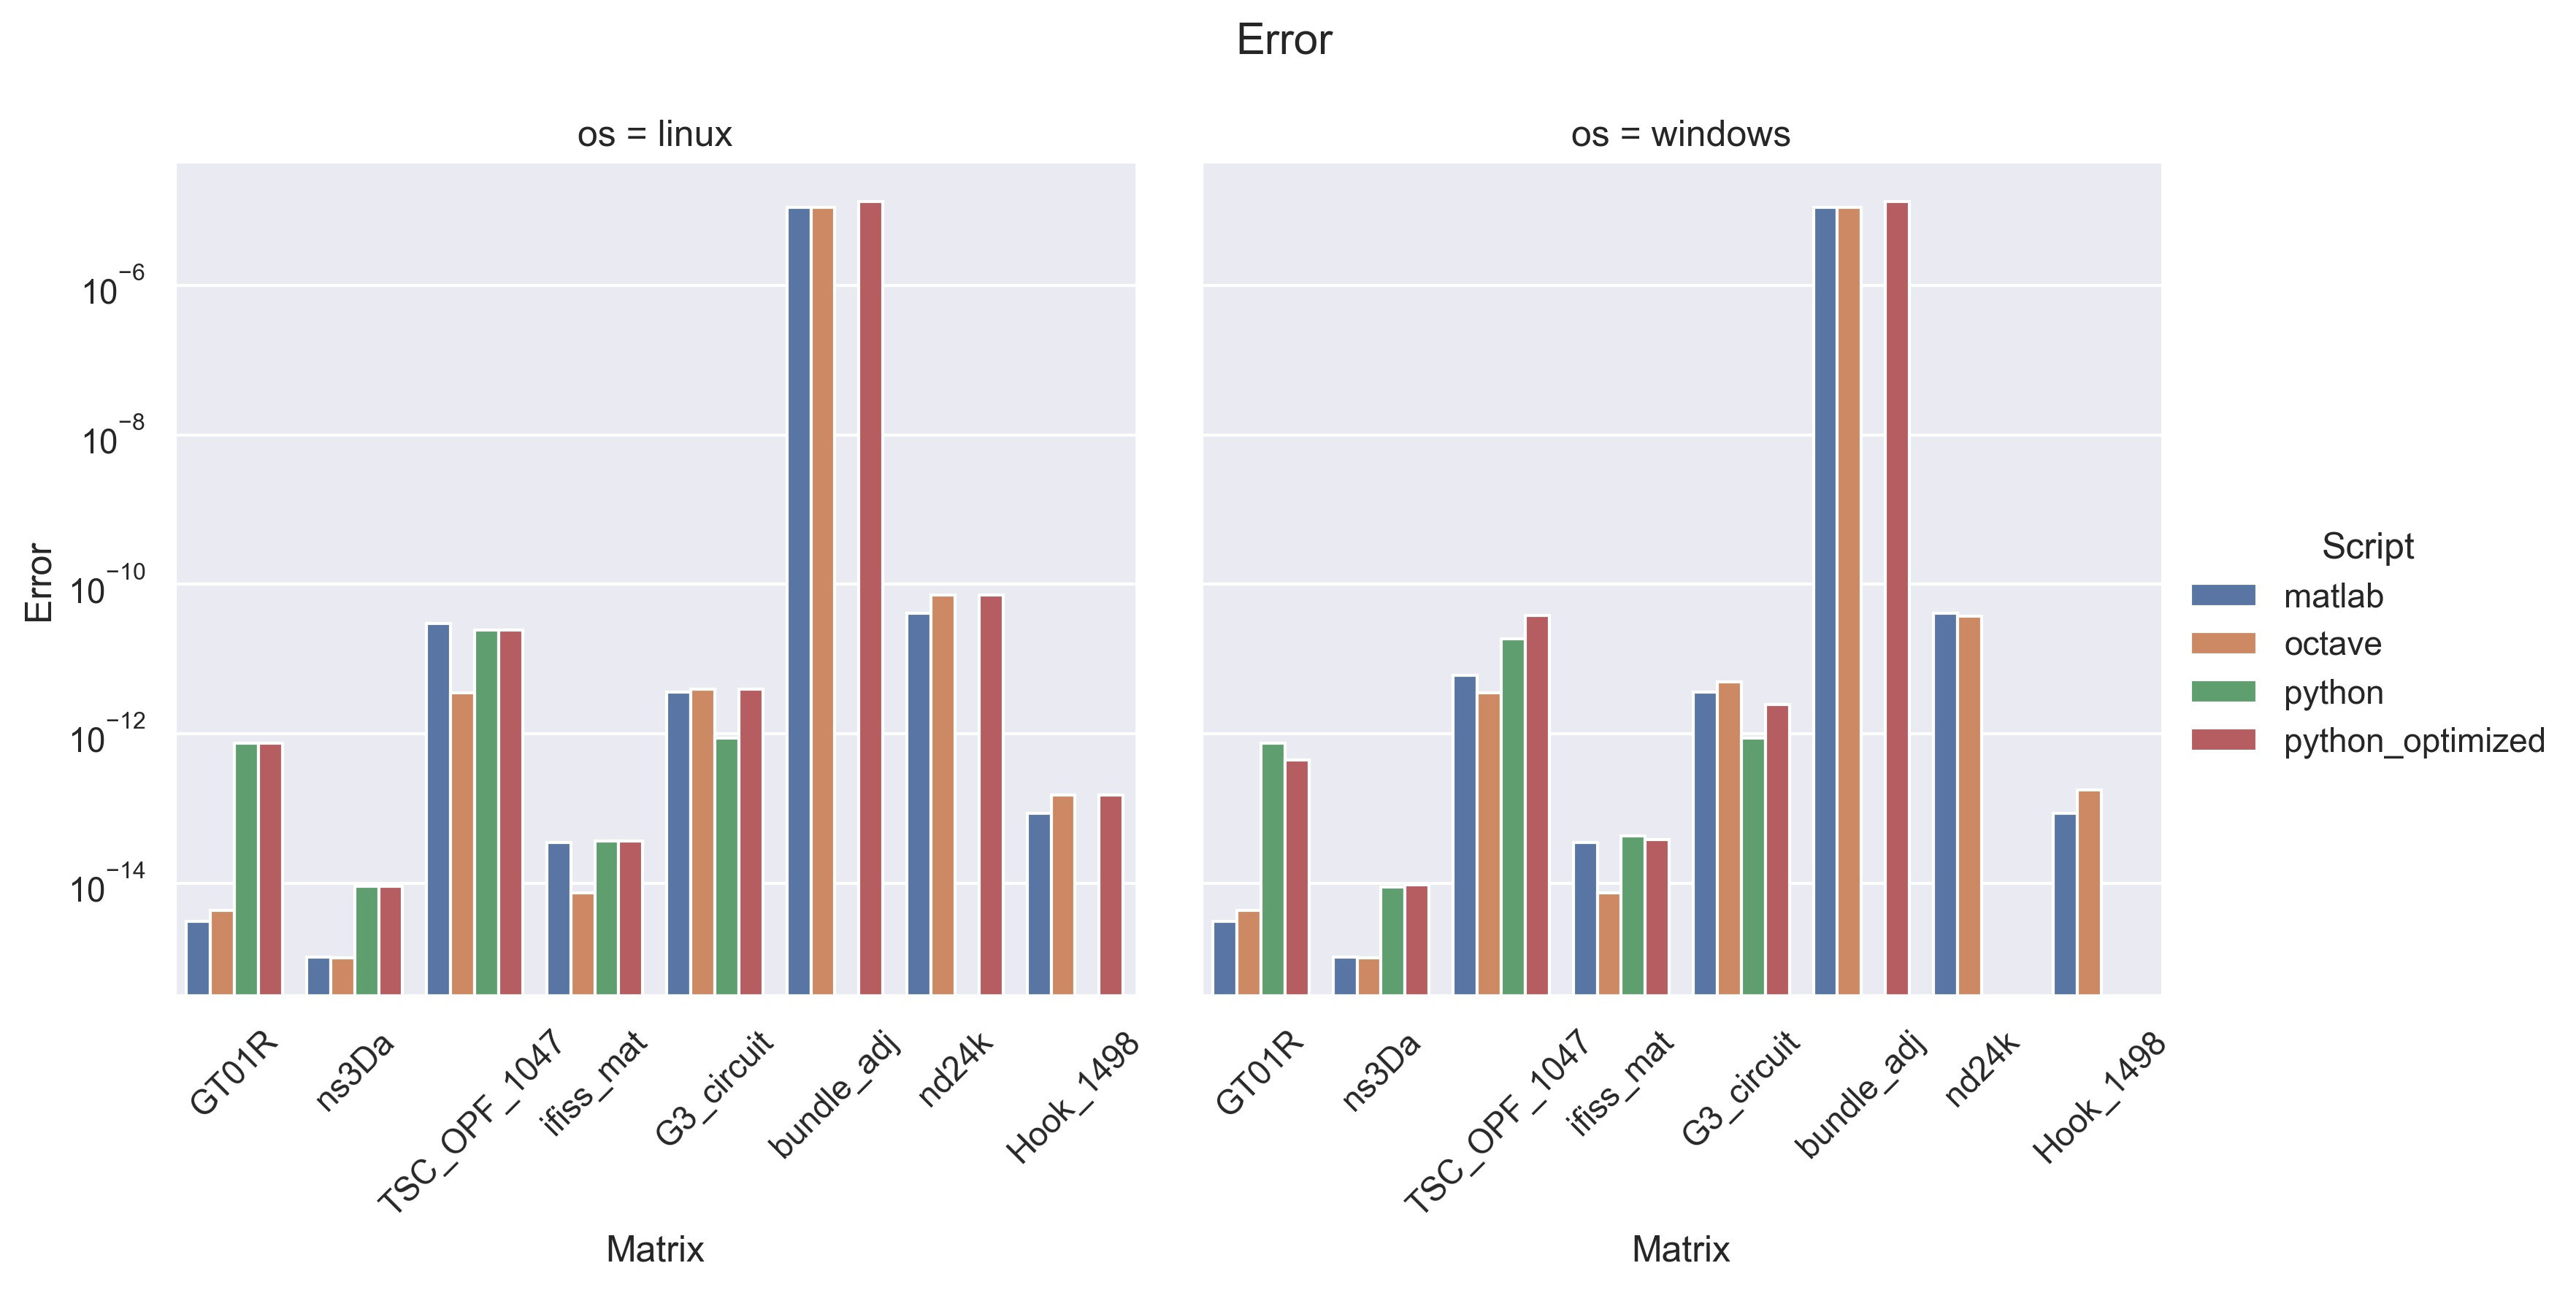
\includegraphics[width=1.35\textheight]{assets/error.jpg}
		\caption{Confronto errore relativo soluzione.}
		\label{fig:error}
	\end{figure}
\end{frame}


\begin{frame}
\frametitle{Codice}
Scipt per il calcolo delle soluzione tra i vari linguaggi di programmazione
\end{frame}


\begin{frame}
	\frametitle{Codice - Matlab}
	\lstinputlisting[language=Matlab, basicstyle=\tiny]{../src/matlab_solver.m}
\end{frame}


\begin{frame}
	\frametitle{Codice - Octave}
	\lstinputlisting[language=Octave, basicstyle=\tiny]{../src/octave_solver.m}
\end{frame}


\begin{frame}
	\frametitle{Codice - Python}
	\lstinputlisting[language=Python, , firstline=8, basicstyle=\tiny]{../src/python_solver.py}
\end{frame}


\begin{frame}
	\frametitle{Codice - Python ottimizzato}
	\lstinputlisting[language=Python, firstline=9, basicstyle=\tiny]{../src/python_solver_optimized.py}
\end{frame}

\section{JPEG}

\subsection{Custom DCT2}

\begin{frame}
\frametitle{Algoritmo usato}
DCT2 fatta con numpy e FFT per confrontare presa da scipy.fft
array crescenti di dimensione $2^i$
\end{frame}

\begin{frame}
\frametitle{Notizie su scipy.fft}
\end{frame}

\begin{frame}
\frametitle{Confronto tra Custom DCT2 e FFT}
grafici - la dct \'e $O(N^3)$, la FFT \'e $O(N^2)$
\end{frame}

\begin{frame}
\frametitle{listato}
\end{frame}

\subsection{Custom JPEG}

\begin{frame}
\frametitle{Algoritmo}
\end{frame}

\begin{frame}
\frametitle{Algoritmo}
\end{frame}

\begin{frame}
\frametitle{Esempi con le immagini proposte}
\end{frame}

\begin{frame}
\frametitle{Sperimentazione}
Momento della presentazione in cui facciamo girare il nostro programma
\end{frame}

\begin{frame}
\frametitle{listato}
\end{frame}

%-----------------------------------------------
% ESEMPI

\begin{frame}
\frametitle{Blocks of Highlighted Text}
\begin{block}{Block 1}
Lorem ipsum dolor sit amet, consectetur adipiscing elit. Integer lectus nisl, ultricies in feugiat rutrum, porttitor sit amet augue. Aliquam ut tortor mauris. Sed volutpat ante purus, quis accumsan dolor.
\end{block}

\begin{block}{Block 2}
Pellentesque sed tellus purus. Class aptent taciti sociosqu ad litora torquent per conubia nostra, per inceptos himenaeos. Vestibulum quis magna at risus dictum tempor eu vitae velit.
\end{block}

\begin{block}{Block 3}
Suspendisse tincidunt sagittis gravida. Curabitur condimentum, enim sed venenatis rutrum, ipsum neque consectetur orci, sed blandit justo nisi ac lacus.
\end{block}
\end{frame}

%------------------------------------------------

\begin{frame}
\frametitle{Multiple Columns}
\begin{columns}[c] % The "c" option specifies centered vertical alignment while the "t" option is used for top vertical alignment

\column{.45\textwidth} % Left column and width
\textbf{Heading}
\begin{enumerate}
\item Statement
\item Explanation
\item Example
\end{enumerate}

\column{.5\textwidth} % Right column and width
Lorem ipsum dolor sit amet, consectetur adipiscing elit. Integer lectus nisl, ultricies in feugiat rutrum, porttitor sit amet augue. Aliquam ut tortor mauris. Sed volutpat ante purus, quis accumsan dolor.

\end{columns}
\end{frame}
%------------------------------------------------

\begin{frame}
\frametitle{Theorem}
\begin{theorem}[Mass--energy equivalence]
$E = mc^2$
\end{theorem}
\end{frame}

%------------------------------------------------

\begin{frame}[fragile] % Need to use the fragile option when verbatim is used in the slide
\frametitle{Verbatim}
\begin{example}[Theorem Slide Code]
\begin{verbatim}
\begin{frame}
\frametitle{Theorem}
\begin{theorem}[Mass--energy equivalence]
$E = mc^2$
\end{theorem}
\end{frame}\end{verbatim}
\end{example}
\end{frame}

%------------------------------------------------

\begin{frame}
\frametitle{Figure}
Uncomment the code on this slide to include your own image from the same directory as the template .TeX file.
%\begin{figure}
%\includegraphics[width=0.8\linewidth]{test}
%\end{figure}
\end{frame}

%------------------------------------------------

\begin{frame}[fragile] % Need to use the fragile option when verbatim is used in the slide
\frametitle{Citation}
An example of the \verb|\cite| command to cite within the presentation:\\~

This statement requires citation \cite{p1}.
\end{frame}

%------------------------------------------------

\begin{frame}
\frametitle{References}
\footnotesize{
\begin{thebibliography}{99} % Beamer does not support BibTeX so references must be inserted manually as below
\bibitem[Smith, 2012]{p1} John Smith (2012)
\newblock Title of the publication
\newblock \emph{Journal Name} 12(3), 45 -- 678.
\end{thebibliography}
}
\end{frame}

%------------------------------------------------

\begin{frame}
\Huge{\centerline{Grazie per l'attenzione}}
\end{frame}

%----------------------------------------------------------------------------------------

\end{document}